%% Преамбула TeX-файла

% 1. Стиль и язык
\documentclass[utf8x]{src/styles/G7-32} % Стиль (по умолчанию будет 14pt)
\usepackage[T2A]{fontenc}
\usepackage[russian]{babel}
% Остальные стандартные настройки убраны в preamble.inc.tex.
\sloppy

% Настройки стиля ГОСТ 7-32
% Для начала определяем, хотим мы или нет, чтобы рисунки и таблицы нумеровались в пределах раздела, или нам нужна сквозная нумерация.
\EqInChapter % формулы будут нумероваться в пределах раздела
\TableInChapter % таблицы будут нумероваться в пределах раздела
\PicInChapter % рисунки будут нумероваться в пределах раздела

% Добавляем гипертекстовое оглавление в PDF
\usepackage[
    bookmarks=true, colorlinks=true, unicode=true,
    urlcolor=black,linkcolor=black, anchorcolor=black,
    citecolor=black, menucolor=black, filecolor=black,
]{hyperref}

% Изменение начертания шрифта --- после чего выглядит таймсоподобно.
% apt-get install scalable-cyrfonts-tex

\IfFileExists{cyrtimes.sty}
{
%    \usepackage{cyrtimespatched}
}
{
% А если Times нету, то будет CM...
}

\usepackage{graphicx}   % Пакет для включения рисунков

% С такими оно полями оно работает по-умолчанию:
% \RequirePackage[left=20mm,right=10mm,top=20mm,bottom=20mm,headsep=0pt]{geometry}
% Если вас тошнит от поля в 10мм --- увеличивайте до 20-ти, ну и про переплёт не забывайте:
\geometry{right=20mm}
\geometry{left=30mm}


% Пакет Tikz
\usepackage{tikz}
\usetikzlibrary{arrows,positioning,shadows}

% Пакет Tikz-uml
\usepackage{tikz-uml}

% Произвольная нумерация списков.
\usepackage{enumerate}

% ячейки в несколько строчек
\usepackage{multirow}

% itemize внутри tabular
\usepackage{paralist,array}

% include pdf documents (itmo titles)
\usepackage{pdfpages}


% Настройки листингов.
% 8 Листинги

\usepackage{listings}

% Значения по умолчанию
\lstset{
    basicstyle= \footnotesize,
    breakatwhitespace=true,% разрыв строк только на whitespacce
    breaklines=true,       % переносить длинные строки
%   captionpos=b,          % подписи снизу -- вроде не надо
    inputencoding=koi8-r,
    numbers=left,          % нумерация слева
    numberstyle=\footnotesize,
    showspaces=false,      % показывать пробелы подчеркиваниями -- идиотизм 70-х годов
    showstringspaces=false,
    showtabs=false,        % и табы тоже
    stepnumber=1,
    tabsize=4,              % кому нужны табы по 8 символов?
    frame=single
}

% Стиль для псевдокода: строчки обычно короткие, поэтому размер шрифта побольше
\lstdefinestyle{pseudocode}{
    basicstyle=\small,
    keywordstyle=\color{black}\bfseries\underbar,
    language=Pseudocode,
    numberstyle=\footnotesize,
    commentstyle=\footnotesize\it
}

% Стиль для обычного кода: маленький шрифт
\lstdefinestyle{realcode}{
    basicstyle=\scriptsize,
    numberstyle=\footnotesize
}

% Стиль для коротких кусков обычного кода: средний шрифт
\lstdefinestyle{simplecode}{
    basicstyle=\footnotesize,
    numberstyle=\footnotesize
}

% Стиль для BNF
\lstdefinestyle{grammar}{
    basicstyle=\footnotesize,
    numberstyle=\footnotesize,
    stringstyle=\bfseries\ttfamily,
    language=BNF
}

% Определим свой язык для написания псевдокодов на основе Python
\lstdefinelanguage[]{Pseudocode}[]{Python}{
    morekeywords={each,empty,wait,do},% ключевые слова добавлять сюда
    morecomment=[s]{\{}{\}},% комменты {а-ля Pascal} смотрятся нагляднее
    literate=% а сюда добавлять операторы, которые хотите отображать как мат. символы
        {->}{\ensuremath{$\rightarrow$}~}2%
        {<-}{\ensuremath{$\leftarrow$}~}2%
        {:=}{\ensuremath{$\leftarrow$}~}2%
        {<--}{\ensuremath{$\Longleftarrow$}~}2%
}[keywords,comments]

% Свой язык для задания грамматик в BNF
\lstdefinelanguage[]{BNF}[]{}{
    morekeywords={},
    morecomment=[s]{@}{@},
    morestring=[b]",%
    literate=%
        {->}{\ensuremath{$\rightarrow$}~}2%
        {*}{\ensuremath{$^*$}~}2%
        {+}{\ensuremath{$^+$}~}2%
        {|}{\ensuremath{$|$}~}2%
}[keywords,comments,strings]

% Подписи к листингам на русском языке.
\renewcommand\lstlistingname{\cyr\CYRL\cyri\cyrs\cyrt\cyri\cyrn\cyrg}
\renewcommand\lstlistlistingname{\cyr\CYRL\cyri\cyrs\cyrt\cyri\cyrn\cyrg\cyri}


% Полезные макросы листингов.
% Любимые команды
\newcommand{\Code}[1]{\textbf{#1}}


\begin{document}

    \frontmatter % выключает нумерацию ВСЕГО; здесь начинаются ненумерованные главы: реферат, введение, глоссарий, сокращения и прочее.

% Команды \breakingbeforechapters и \nonbreakingbeforechapters
% управляют разрывом страницы перед главами.
% По-умолчанию страница разрывается.

% \nobreakingbeforechapters
% \breakingbeforechapters

    \setcounter{page}{6}

    \tableofcontents

    \Abbreviations %% Список обозначений и сокращений в тексте
\begin{description}
    \item[ЭВМ] Электронно-вычислительная машина
    \item[ВС] Вычислительная система
    \item[ПО] Программное обеспечение
    \item[DevOps] Development & Operations, <<Разработка и Эксплуатация>>
    \item[SaaS] Software as a Service, <<Программное обеспечение как услуга>>
    \item[IaC] Infrastructure as Code, <<Инфраструктура как код>>
    \item[CI/CD] Continuous Integration/Continuous Deployment, <<Продолжительная интеграция/Продолжительная развёртка>>
    \item[VCS] Version Control System, <<Система контроля версий>>
    \item[CLI] Command Language Interface, <<Интерфейс командной строки>>
\end{description}

%%% Local Variables:
%%% mode: latex
%%% TeX-master: "rpz"
%%% End:


    \Introduction

Веб технологии широко распространились в нашем мире и на сегодняшний день почти каждая ВС взаимодействует со всемирной паутиной.
В свою очередь, поддержка и разработка наиболее популярной архитектуры <<Клиент-Сервер>> таких систем требует существенных временных затрат, поскольку уже с самого начала проектирования требуется решить ряд следующих задач:

\begin{itemize}
    \item вертикальное и горизонтальное масштабирование системы,
    \item доставка обновлений сервиса на рабочие ЭВМ,
    \item управление окружением ВС,
    \item осуществления контроля качества поступающих изменений,
    \item управление версиями ВС,
    \item бесшовное развёртывание отдельных компонентов системы,
    \item оперативная загрузка срочных исправлений.
\end{itemize}

Для решения данных задач в современном мире применяется DevOps методология разработки ПО\cite{projectPhoenix}.
Основная идея заключается в предоставлении удобных инструментов связи разработчиков, системных администраторов и не только.

DevOps включает в себя множество различных технологий, среди которых можно выделить
SaaS --- это облачное решение при использовании \cite{cd}
которого, пользователь получает доступ к сервису, как правило, через браузер или по API;
IaC --- это процесс управления и позиционирования дата центров и серверов с помощью машиночитаемых файлов определений,
созданный как альтернатива физическому конфигурированию оборудования и оперируемым человеком инструментам;
а так же CI/CD --- это методология обеспечения оперативности вывода новой функциональности продукта и повышение качества разрабатываемого решения\cite{ciCd}.

Теперь, вместо того, чтобы запускать сотню различных файлов конфигурации,
достаточно запускать скрипт, который управляет инфраструктурой и масштабированием системы.

Несмотря на это, для ввода в рабочий процесс всё равно необходима дополнительная разработка механизмов развёртки,
начиная от описания файлов конфигураций до разработки дополнительных порграммных средств.

В зависимости от решаемых задач и условий эксплуатации разработчиками выбираются конкретные DevOps инструменты.

Разрабатываемая в рамках данной работы система автоматизации управления жизненным циклом веб-сервиса,
согласно техническому заданию, должна отвечать следующим требованиям:

\begin{itemize}
    \item использовать современные DevOps методологии,
    \item взаимодействие с конечным пользователем по методологии SaaS,
    \item возможность добавления в систему не описанных заранее сервисов по методологии IaC,
    \item использование методологии CI/CD для взаимодействия с инфраструктурой и организации контроля качества,
    \item наличие конфигурации прав доступа (приватизации исходного кода),
    \item наличие хранилища пакетов и образов,
    \item стоимость установки и обслуживания системы --- не более 2 500 рублей за установку 2 500 рублей в месяц за обслуживание на момент написания данной работы.
\end{itemize}

Поставленные требования определяют предмет исследования:

Простое и доступное в установке и поддержке ПО для автоматизации управления жизненным циклом веб-сервиса\cite{vkrsen}.

Объект исследования: ПО, задействованные и которые могут быть использованы для автоматизации управления жизненным циклом веб-сервиса.

При проведении исследований были просмотрены 20 источников, в том числе 11 электронных ресурсов, что отражено в библиографическом списке.
При написании выпускной квалификационной работы (ВКР) из библиографического списка использовано 5 источников.

ВКР состоит из введения, основной части, включающей четыре главы, заключения и приложений.
В ВКР содержится 31 страница основного текста, 11 рисунков, 3 таблицы и 0 приложений.

    \mainmatter % это включает нумерацию глав и секций в документе ниже

    \chapter{ОБЗОР СУЩЕСТВУЮЩИХ СИСТЕМ АВТОМАТИЗАЦИИ УПРАВЛЕНИЯ ЖИЗНЕННЫМ ЦИКЛОМ ВЕБ-СЕРВИСА}
\label{cha:analysis}

\section{Система контроля версий}

Для корректного формулирования требований к разрабатываемому комплексу автоматизации управления жизненным циклом веб-сервиса,
необходимо проанализировать и сравнить характеристики схожих по назначению решений, применяемых в данный момент на архитектуре <<Клиент-Сервер>>,
либо по своим характеристикам подходящих для такого применения.

Рассматривая рынок развёртки программного обеспечения, стоит начать с такого ключевого элемента, как VCS.

Наиболее популярной системой контроля версий на момент написания работы является git\cite{web:git:book}.
Git --- система управления версиями программного обеспечения с распределенной архитектурой.
В отличие от некогда популярных систем вроде CVS и Subversion (SVN),
где полная история версий проекта доступна лишь в одном месте,
в Git каждая рабочая копия кода сама по себе является репозиторием.
Это позволяет всем разработчикам хранить историю изменений в полном объеме.
Разработка в Git ориентирована на обеспечение высокой производительности, безопасности и гибкости распределенной системы.

\section{Git хостинг}

Сам по себе git предоставляет только инструменты для локальной разработки и имеет весьма ограниченный функционал.
Для работы в большинстве случаев выбирается SaaS Git хостинг исходного кода.
Такие сервисы предоставляют удобный масштабируемый хостинг для Git-репозиториев с веб-интерфейсом для просмотра и редактирования кода,
а также гибкими настройками доступа.
Современные и простые способы организации процессов CI/CD и решения самых разных задач с их помощью.

В настоящее время на рынке имеется несколько лидерующих представителей, отличающихся в основном стоимостью и набором дополнительных инструментов\cite{web:git-reps:rating}.

Наиболее популярным из таких хостингов является GitHub от международной компании Microsoft.
Для проектов с открытым исходным кодом сервис бесплатен.
Функции приватизации и контроля доступа для команд предоставляются за отдельную плату.
Для развёртки проектов по методологии CI/CD, GitHub предоставляет инструмент Actions.
Хранилище образов и пакетов предоставляется с ограничением и только проектам с открытм исходным кодом.
В целом, данный хостинг лучше всего подходит для таких проектов и редко используется командами разработчиков в коммерческой сфере деятельности.

Следующим из таких хостингов является Bitbucket\cite{web:bitbucket} от австралийской компании Atlassian.
Данный хостинг более акцентирован на коммерческую разработку и предоставляет функции приватизации бесплатно для небольших команд.
Возможности CI/CD аналогичны GitHub Actions, только предоставляются продуктом Bamboo.
Хранилище образов и пакетов отсутствует.
Bitbucket следует рассматривать, как альтернативу GitHub только для коммерческой разработки\cite{web:github:docs}.

Одним из наиболее подходящих хостингов является GitLab от украинских разработчик (ныне зарубежной компании GitLab Inc).
Ключевой особенностью является то, что этот сервис изначально разрабтывался,
как полноценная система для управления жизненным циклом программного обеспечения на всех этапах разработки.
Благодаря этому в нём реализовано большинство основных функций для обеспечения полноценного рабочего окружения по методологии CI/CD.
Бесплатно сервис предоставляет, как приватизацию и управление доступом к исходному коду, так и хранилища образов и пакетов.
Возможности непрерывной интеграции и доставки включают в себя отчеты о тестировании в реальном времени, параллельное выполнение, локальный запуск скриптов, поддержку Docker\cite{web:gitlab}.

Так же был рассмотрен продукт от разработчиков из Санкт-Петербурга (международной компании JetBrains) --- Space\cite{web:space:docs}.
Данное решение является интегрированной средой для командной работы, которая включает управление исходным кодом, постановку и работу над задачами, управление командами разработчиков и инструменты коммуникации.
Все функции Space так же предоставляет бесплатно, но с ограничениями в разумных пределах, подходящими небольшим командам разработчиков.
Несмотря на большое количество возможностей, данный продукт существует на рынке сравнительно небольшое количество времени и большинство ключевых функций ещё не реализовано.

\begin{center}
    \begin{longtable}{|p{0.4\textwidth}|c|c|c|c|}
        \caption{Сравнение Git хостингов}
        \label{tab:git-hostings}
        \hline
        Функция                             & GitHub          & BitBucket   & GitLab    & Space \\
        \hline
        Настройки доступа                   & Огр.            & +           & +         & +     \\
        Хранилище контейнеров и пакетов     & 500 Mb          & -           & 10 Gb     & 10 Gb \\
        Инструменты CI/CD                   & Огр.            & Огр.        & Огр, +    & Огр.  \\
        Количество пользователей            & Неогр.          & 5           & Неогр.    & Неогр.\\
        \hline
    \end{longtable}
\end{center}

\section{Инструмент оркестрации}

Помимо git хостинга данному проекту так же потребуется механизм масштабирования системы.
Технология контейнеризации (Docker) позволяет запускать приложения в отдельных независимых средах --- контейнерах.
Они упрощают развертывание приложений, изолируют их друг от друга и ускоряют разработку.
Но когда контейнеров становится слишком много, ими трудно управлять.
Тут на помощь приходят IaC системы оркестрации \cite{likeGoogle}.

У Docker есть стандартный инструмент оркестрации --- Docker Swarm.
Он поставляется вместе с Docker, довольно прост в настройке и позволяет создать кластер в кратчайшие сроки.
Из минусов следует отметить узкую функциональность: возможности ограничены Docker API.
Это значит, что Swarm способен сделать лишь то, что позволяют возможности Docker\cite{fasterDevOps}.

Альтернативным решением является Kubernetes --- это универсальное средство для создания распределенных систем.
Это комплексная система с большим количеством возможностей, разработка и поддержка которой самостоятельно значительно трудозатратна.
Kubernetes мощный инструмент, имеющий много возможностей, которые позволяют строить действительно комплексные распределенные системы.
К минусам относится управление, как оно использует отдельный набор команд и инструментов, несовместимых с Docker CLI\cite{web:docker-kubernetes}.
Гибкость данного решения излешне и лишь затруднит введение проекта в рабочее состояние в контексте данной работы.

Подводя итоги исследования доступных решений систем автоматизации управления жизненным циклом веб-сервисов, можно сделать следующие выводы:
\begin{itemize}
    \item анализ источников показывает, что на рынке отсутствуют подходящие под требования проектируемой системы готовые решения,
    позволяющие осуществлять дальнейшие доработки системы под конкретные задачи;
    \item анализ использованных источников показывает, что цели и задачи работы возможно реализовать на основе Git хостинга GitLab,
    разработав программные механизны части системы.
    Правильный выбор сервисных компонентов системы позволит выполнить требования технического задания и достигнуть цели работы.
\end{itemize}

%%% Local Variables:
%%% mode: latex
%%% TeX-master: "rpz"
%%% End:

    \chapter{Конструкторский раздел}
\label{cha:design}

В данном разделе проектируется новая всячина.

\section{Архитектура всячины}

\paragraph{Проверка} параграфа. Вроде работает.
\paragraph{Вторая проверка} параграфа. Опять работает.

Вот.

\begin{itemize}
    \item Это список с <<палочками>>.
    \item Хотя он и не по ГОСТ, кажется.
\end{itemize}

\begin{enumerate}
    \item Поэтому для списка, начинающегося с заглавной буквы, лучше список с цифрами.
\end{enumerate}

Формула \ref{F:F1} совершено бессмысленна.

%Кстати, при каких-то условиях <<удавалось>> получить двойный скобки вокруг номеров формул. Вопрос исследуется.

\begin{equation}
    a= cb
    \label{F:F1}
\end{equation}


Окружение \texttt{cases} опять работает (см. \ref{F:F2}), спасибо И. Короткову за исправления..


\begin{equation}
    a= \begin{cases}
           3x + 5y + z, \mbox{если хорошо} \\
           7x - 2y + 4z, \mbox{если плохо}\\
           -6x + 3y + 2z, \mbox{если совсем плохо}
    \end{cases}
    \label{F:F2}
\end{equation}

\section{Подсистема всякой ерунды}

Культурная вставка dot-файлов через утилиту dot2tex (рис.~\ref{fig:fig02}).

\begin{figure}
% [width=0.5\textwidth] --- регулировка ширины картинки
    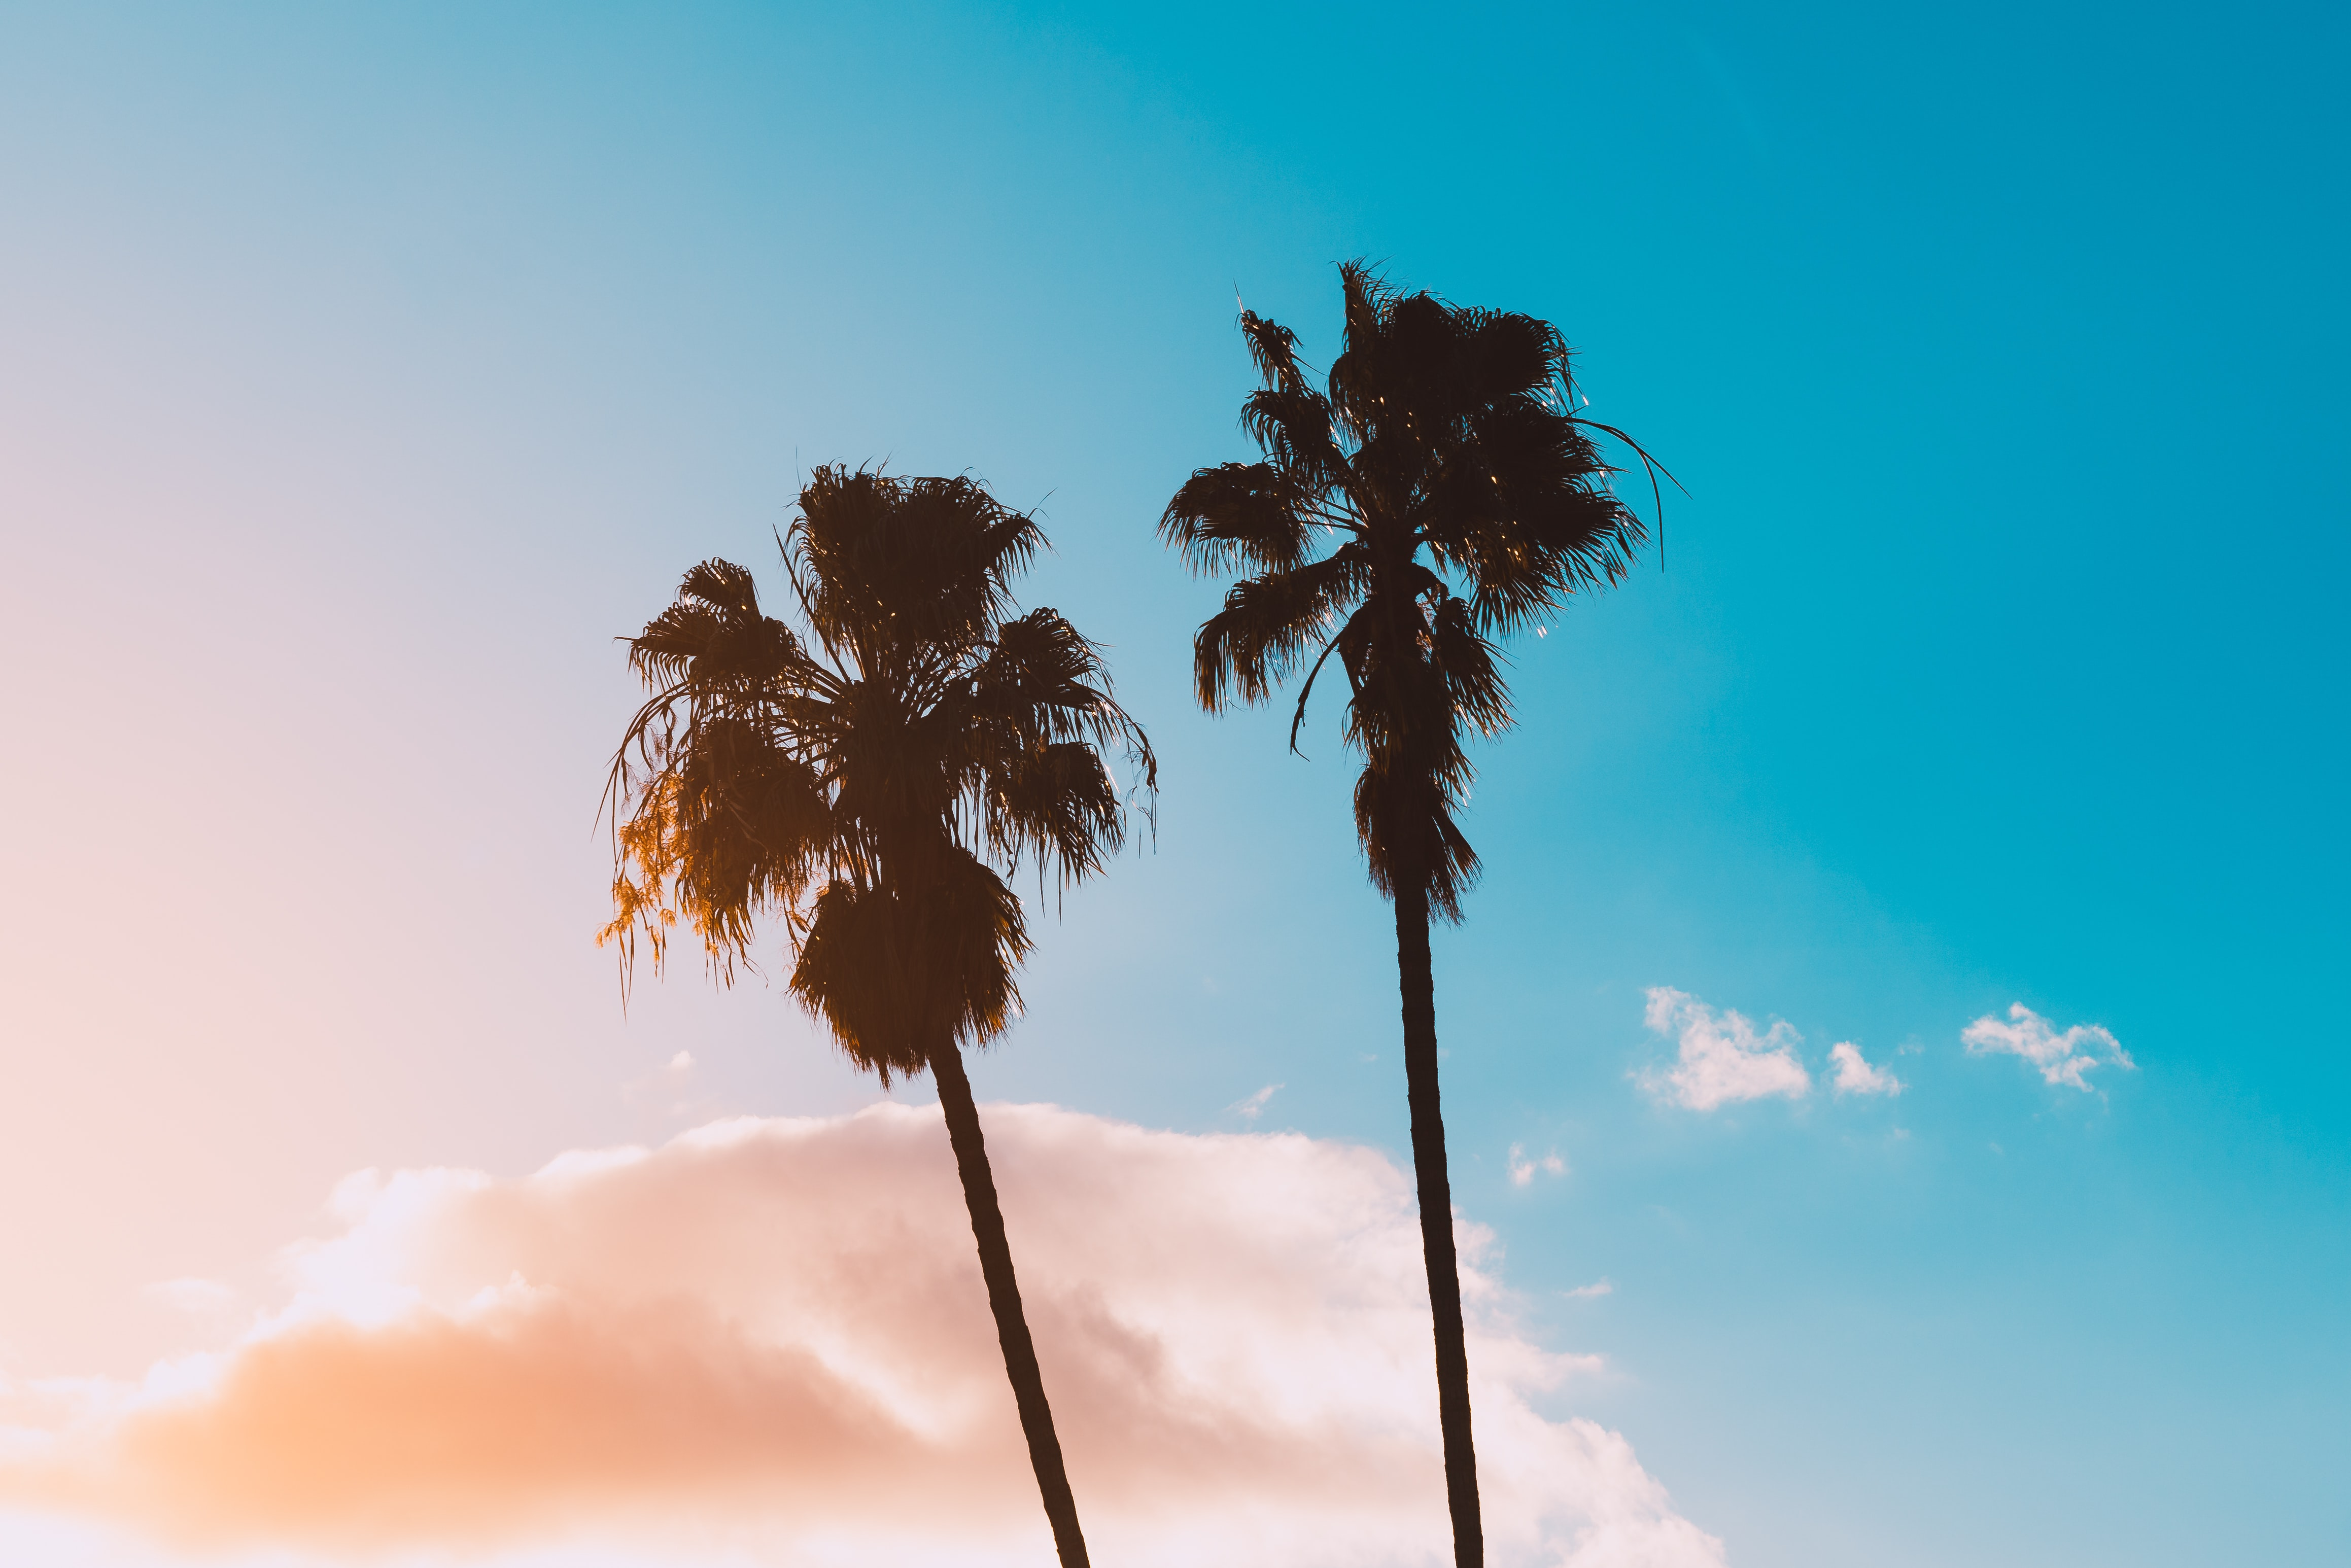
\includegraphics{figures/pic01}
    \caption{Рисунок}
    \label{fig:fig02}
\end{figure}

\begin{figure}
    \centering
    \begin{tikzpicture}
        \begin{umlsystem}[x=4]{system}{Автоматизация жизненным циклом веб-сервиса}
            \umlusecase[width=3cm]{Управление правами доступа}
            \umlusecase[y=-4, width=3cm]{Управление развёрткой}
            \umlusecase[x=6, width=3cm]{Получить актуальную версию веб-сервиса}
            \umlusecase[x=6, y=-4, width=3cm]{Получить тестовую версию веб-сервиса}
        \end{umlsystem}

        \umlactor{Разработчик}{developer}
        \umlactor[y=-3]{Админнистратор}{admin}
        \umlactor[x=14]{Пользователь}{user}
        \umlactor[x=14,y=-3]{Сотр. отдела качества}{qa}

%        \umlassoc{user}{usecase-1}

%        \umlinherit{subuser}{user}
%        \umlassoc{user}{usecase-1}
%        \umlassoc{subuser}{usecase-2}
%        \umlassoc{subuser}{usecase-3}
%        \umlinherit{usecase-2}{usecase-1}
%        \umlVHextend{usecase-5}{usecase-4}
%        \umlinclude[name=incl]{usecase-3}{usecase-4}
    \end{tikzpicture}
    \caption{UML диаграмма}
    \label{fig:fig03}
\end{figure}


\subsection{Блок-схема всякой ерунды}

\subsubsection*{Кстати о заголовках}

У нас есть и \Code{subsubsection}. Только лучше её не нумеровать.

Проводя обзор доступных на рынке git хостингов, можно сделать вывод, что наиболее распространенным git хостингом на сегодняшний день является хостинг компании GitLab Inc.
К тому же, по соотношению цена-функционал хостинг этой компании существенно обходит конкурентов.
Также, к существенному преимуществу можно отнести наличие обширного сообщества пользователей и разработчиков программных решений на основе git хостинга GitLab,
что позволяет иметь доступ к множеству готовых решений и получать помощь в разработке при необходимости.

Для реализации поставленной в данной работе задачи гибкость настройки всей инфраструктуры окружения не требуется, а также ставится в приоритет скорость ввода в рабочее состояние.
Поэтому в качестве оркестратора вместо гибкости Kubernetes был выбран Docker Swarm.
Но так как в данной работе делаеся акцент на гибкость всей системы, то далее будет рассмотрена описание конфигурации для использования с Kubernetes, не считая уставноку и настройку самого кластера.
Для работы будет подготовлена одна вершина Docker Swarm в статусе мэнеджер, поскольку более не требуется на данном этапе.

Как было сказано ранее, для развёртки в работе используется Docker, поэтому необходим простой инструмент удлаенного доступа к сокету Docker сервиса на рабочем сервере.
Для этих целей будет использоваться GitLab Runner с установленным исполнителем задач Docker.
Кратко описать работу ранера можно следующим образом: раннер запускается в отдельном контейнере с добавленным volume на сокет Docker,
таким образом получается избежать достаточно сложного и нелесообразного запуска Docker внутри Docker,
так как в этом случае раннер получает доступ напрямую к сокету Docker сервера.
Данное решение имеет потенциальную проблему с безопасностью, поскольку если злоумышленник получит доступ к описанию задач GitLab CI/CD, то он сможет запускать на рабочем сервере любое ПО.
Для избежания данной проблемы будут установлены настройки доступа внутри GitLab.
Так же для избежания потери полезного времени работы ранера, необходимо будет произвести настройку кэша ранера.
Ключевой настройкой явлется политика загрузки образов для задач, поскольку по умолчанию ранер в любом случае будет загружать образ из регистра, даже если образ представлен локально.
Согласно требованиям ранер должен будет запускать минимум три задачи за единицу времени, данное значение будет отражено в конфигурации на этапе реализации.

Автоматизация контроля качества будет реализована путём запуска описанных разработчиками тестовых сценариев внутри Pipelines.
Отчёты по прохождению сценариев будут представлены в веб интерфейсе GitLab путём интеграции с CI/CD.

Для контроля версий будет использована модель ветвления git flow со следующими окружениями:

\begin{itemize}
    \item develop --- инсценировка рабочего окружения веб серсива для разработчиков,
    \item testing --- окружение для проведения ручного тестирования,
    \item release --- рабочее окружение сервиса для реальных пользователей.
\end{itemize}

Основная проблема заключается в обновлении пакетов зависимостей проекта, поскольку для обновления необходимо пройти засимимым сервисам и построить граф.
Для решения этой проблемы будет разработано программное решение на базе CI/CD c применением bash скриптов при помощи package.json файлов веб сервиса.

Для проведения тесирования был составлен план содержащий набор ключевых функция для тестирвоания.
Подробнее план представлен в виде таблице с описанием сценариев, входных данных и ожидаемого результата в тестке работы ВКР.


%%% Local Variables:
%%% mode: latex
%%% TeX-master: "rpz"
%%% End:

    \chapter{РЕАЛИЗАЦИЯ СИСТЕМЫ АВТОМАТИЗАЦИИ УПРАВЛЕНИЯ ЖИЗНЕННЫМ ЦИКЛОМ ВЕБ-СЕРВИСА}
\label{cha:impl}

\section{Подготовка GitLab}

Перед реализацией необходимо произвести базовую настройку окружения.
Для этого был зарегистрирован GitLab аккаунт, установлен SSH ключ и создана группа проекта.
Результаты создания группы представлены на рисунке \ref{fig:group-ready}.

\begin{figure}[ht]
    \centering
    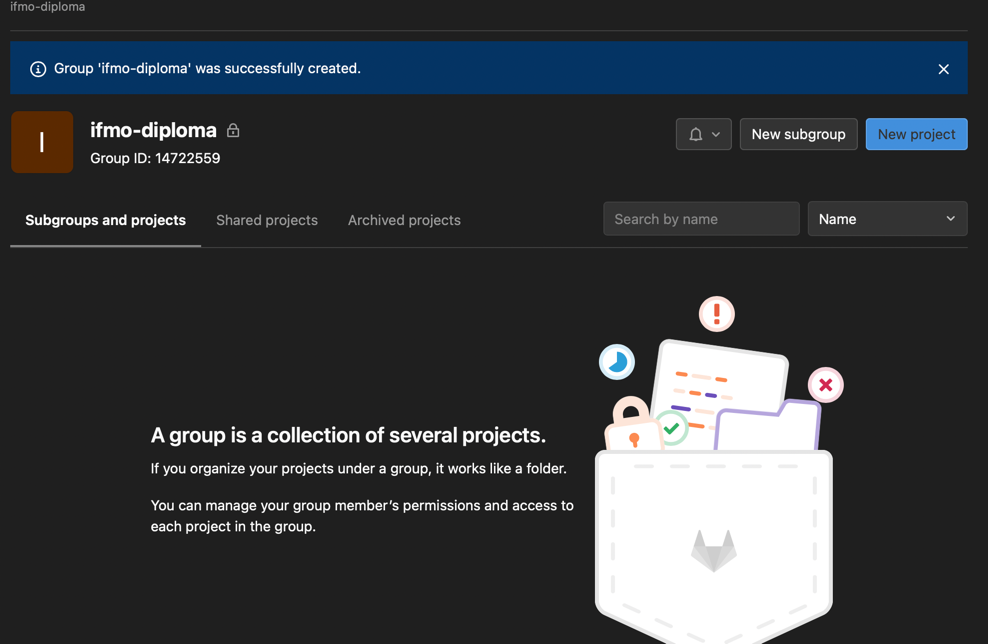
\includegraphics[scale=0.4]{src/figures/group-ready}
    \caption{Скриншот создания группы в GitLab}
    \label{fig:group-ready}
\end{figure}

Следующим этапом было произведено создание необходимых репозиториев с последующей загрузкой исходного кода предоставленного для работы веб-сервиса:

\begin{itemize}
    \item web-client --- репозиторий для хранения исходного кода веб-клиента проекта,
    \item api --- репозиторий для хранения исходного кода API проекта.
    \item node-packages --- репозиторий для хранения исходного кода общих npm зависимостей проекта.
\end{itemize}

Так же в корне каждого репозитория был загружен Dockerfile для развёртывания данного сервиса.
Так как в качестве модели ветвления была выбрана модель git flow, то так же были подготовлены соответствующие ветки в репозиториях под разные окружения: develop, testing и release.
Установка доступа к данным репозиториям предоставляется только разработчикам данных программных решений в целях безопасности.

Подготовка хранилищ npm\cite{web:npm:docs} пакетов и Docker образов не требуется, так как GitLab берёт на себя данную ответственность и не требует дополнительных действий от пользователя.

На следующем этапе был подготовлен репозиторий deployment для хранения общих скриптов и конфигураций окружения и развёртывания.
Установка доступа к этому репозиторию предоставляется только команде обеспечения развёртывания в целях безопасности.
Результаты создания репозиториев представлены на рисунке \ref{fig:reps-ready}.

\begin{figure}[ht]
    \centering
    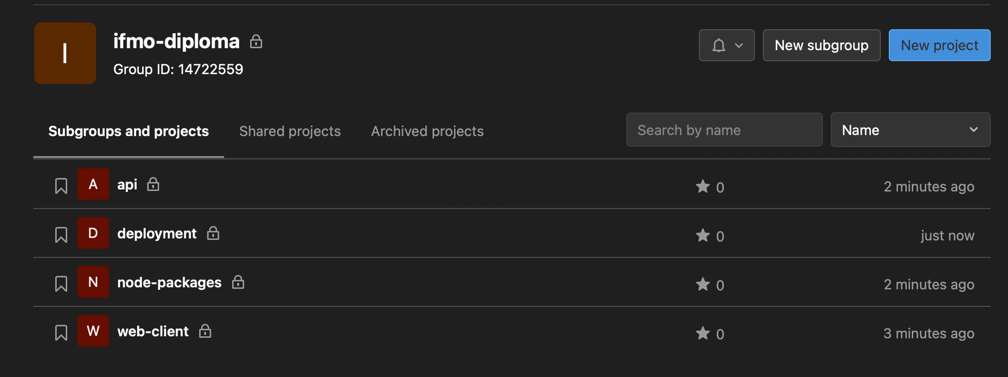
\includegraphics[scale=0.4]{src/figures/reps-ready}
    \caption{Скриншот создания репозиториев в GitLab}
    \label{fig:reps-ready}
\end{figure}

\section{Установка кластера Docker Swarm}

Следующим этапом был установлен и настроен Docker Swarm кластер.

Для этого на рабочей системе было произведено открытие необходимых портов в операционной системе\cite{linuxPocket}:
\begin{lstlisting}[language=bash,caption={Открытие портов в Linux}]
$ sudo ufw allow 2377
$ sudo ufw allow 7946
$ sudo ufw allow 4789
\end{lstlisting}

Дальше была произведена инициализация кластера на сервере:
\begin{lstlisting}[language=bash,caption={Инициализация кластера}]
$ docker swarm init --advertise-addr 192.168.1.101
  Swarm initialized: current node (dxn1zf6l61qsb1josjja83ngz) is now a manager.
  To add a worker to this swarm, run the following command:
    docker swarm join --token <token> 192.168.1.101:2377
  To add a manager to this swarm, run 'docker swarm join-token manager' and follow the instructions.
\end{lstlisting}

В данном этапе нет необходимости при использовании Kubernetes.

\section{Установка и настройка GitLab Runner}

После была произведена установка и настройка GitLab Runner на рабочем сервере.
В качестве дистрибутива на этапе проектирования был выбран Docker, как самый быстрый и удобный.
После установки необходимо зарегистрировать GitLab Runner, для этого на странице настроек CI/CD группы в GitLab был получен регистрационный токен.
Конфигурация runner производится путём редактирования config.toml\cite{web:gitlab:docs} файла в соответствии с этапом проектирования, основными настройками являются:

\begin{itemize}
    \item Установка executor --- docker executor,
    \item Установка volumes --- /var/run/docker.sock\cite{web:docker:docs},
    \item Установка pull-policy --- if-not-present,
    \item Установка concurrent --- 3.
\end{itemize}

На данном этапе runner полностью готов к работе и ожидает входящих задач.

\section{Описание CI/CD конфигураций}

На следующем этапе необходимо подготовить общие для работы сервисов конфигурации запуска, которые будут храниться в репозитории deployment:

\begin{itemize}
    \item build.yaml --- набор универсальных задач, предназначенный для сборки Docker образа и последующей загрузки в регистр контейнеров,
    \item publish.yaml --- набор универсальных задач, предназначенный для оповещения кластера об обновлении сервиса для загрузки новой версии,
    \item publish-api.yaml --- расширенная версия publish.yaml, содержащая дополнительные задачи для проведения миграция базы данных в случае необходимости,
\end{itemize}

Одним из наиболее интересных файлов конфигураций является .gitlab-ci.yaml, поскольку в нём содержится основная логика управления развёрткой веб-сервиса.
На данных строчках содержится автоматическое подключение к кластеру Docker образов без с учётом риска передачи паролей через переменные окружения.
Так же в данных строчках содержится описание стадий задач, необходимых для развёртки сервиса api.
Пример приведён на листинге \ref{lst:api-tasks}.

\lstinputlisting[language=yaml,caption=Задачи сервиса api (\Code{deployment/.gitlab-ci.yml}),label=lst:api-tasks]{src/listings/api-tasks.yaml}

Данная задача используется для безопасного обновления конкретного сервиса по его названию и названию окружения, которая добавляется в линию только при указании значения названия сервиса и ветки.
Пример приведён на листинге \ref{lst:update-a-service}.

\lstinputlisting[language=yaml,caption=Обновление сервиса (\Code{deployment/.gitlab-ci.yml}),label=lst:update-a-service]{src/listings/update-a-service.yaml}

В конце файла содержится задача, условием запуска которой является отсутствие названия сервиса и веток.
Данная задача используется для экстренного перезапуска веб-сервиса.
Пример приведён на листинге \ref{lst:update-service}.

\lstinputlisting[language=yaml,caption=Перезапуск веб-сервиса (\Code{deployment/.gitlab-ci.yml}),label=lst:update-service]{src/listings/update-service.yaml}

Далее была произведена конфигурация на уровне сервисов компонентов, в репозитории api и web-client были добавлены конфигурации CI/CD путём создания .gitlab-ci.yml файла, содержащего основные задачи.

Для репозитория node-packages были описаны задачи с использованием CLI lerna, которая предназначена для организации работы моно-репозитория.
Использование этой библиотеки обусловлено большим сообществом разработчиков и открытостью исходного кода.
Данная программа обновляет версии библиотек при помощи построения и обхода графа зависимостей, построенного на основании package.json файлов.
Пример данного графа в условиях данного веб-сервиса приведён на рисунке \ref{fig:dependency-graph}.

\begin{figure}[ht]
    \centering
    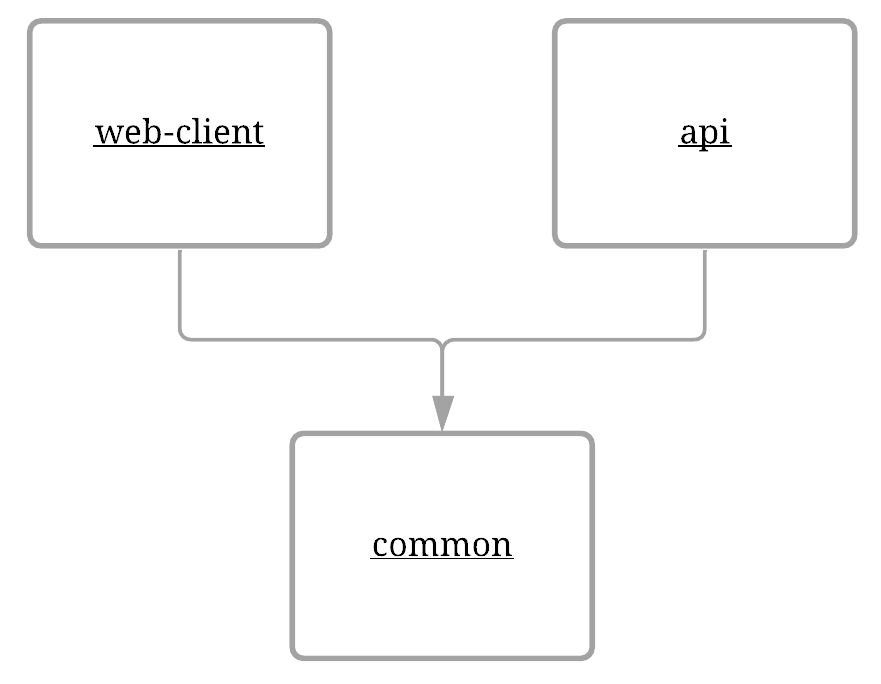
\includegraphics[scale=0.4]{src/figures/dependency-graph}
    \caption{Граф зависимостей компонентов веб-сервиса}
    \label{fig:dependency-graph}
\end{figure}

\section{Развёртка сервисов внутри кластера}

Завершающим этапом реализации является описание конфигурационных файлов Docker Swarm.
Для этого в настройках CI/CD репозитория deployment были добавлены переменные окружения (секреты) на все рабочие окружения (develop, testing и release),
содержащие аргументы сервисов компонентов системы (доступы к базе данных, секрет ключа авторизации и так далее)\cite{kuberForDevOps}.
Аналогично были добавлены Docker Swarm конфигурационные файлы под каждый окружения:

\begin{itemize}
    \item develop --- каждый сервис запускается на сервере в одном экземпляре, ресурсы сервера сильно ограничены во избежание лишней нагрузки,
    \item testing --- аналогичен develop, только используется для целей ручного тестирования веб-сервиса,
    \item release --- web-client запускается в одном экземпляре, база данных и api запускаются в трёх, большая часть ресурса отведена под эти сервисы.
\end{itemize}

На листинге \ref{lst:api-services} приведён пример части конфигурационного файла Docker Swarm для запуска сервиса api.

\lstinputlisting[language=yaml,caption=Сервисы api (\Code{deployment/docker-compose.master.yaml}),label=lst:api-services]{src/listings/api-services.yaml}

На листинге \ref{lst:web-client-services} приведён пример части конфигурационного файла Docker Swarm для запуска сервиса web-client.

\lstinputlisting[language=yaml,caption=Сервисы web-client (\Code{deployment/docker-compose.master.yaml}),label=lst:web-client-services]{src/listings/web-client-services.yaml}

В итоге веб-сервис был развёрнут, пример открытия веб страницы приведён на рисунке \ref{fig:app-screen}.

\begin{figure}[ht]
    \centering
    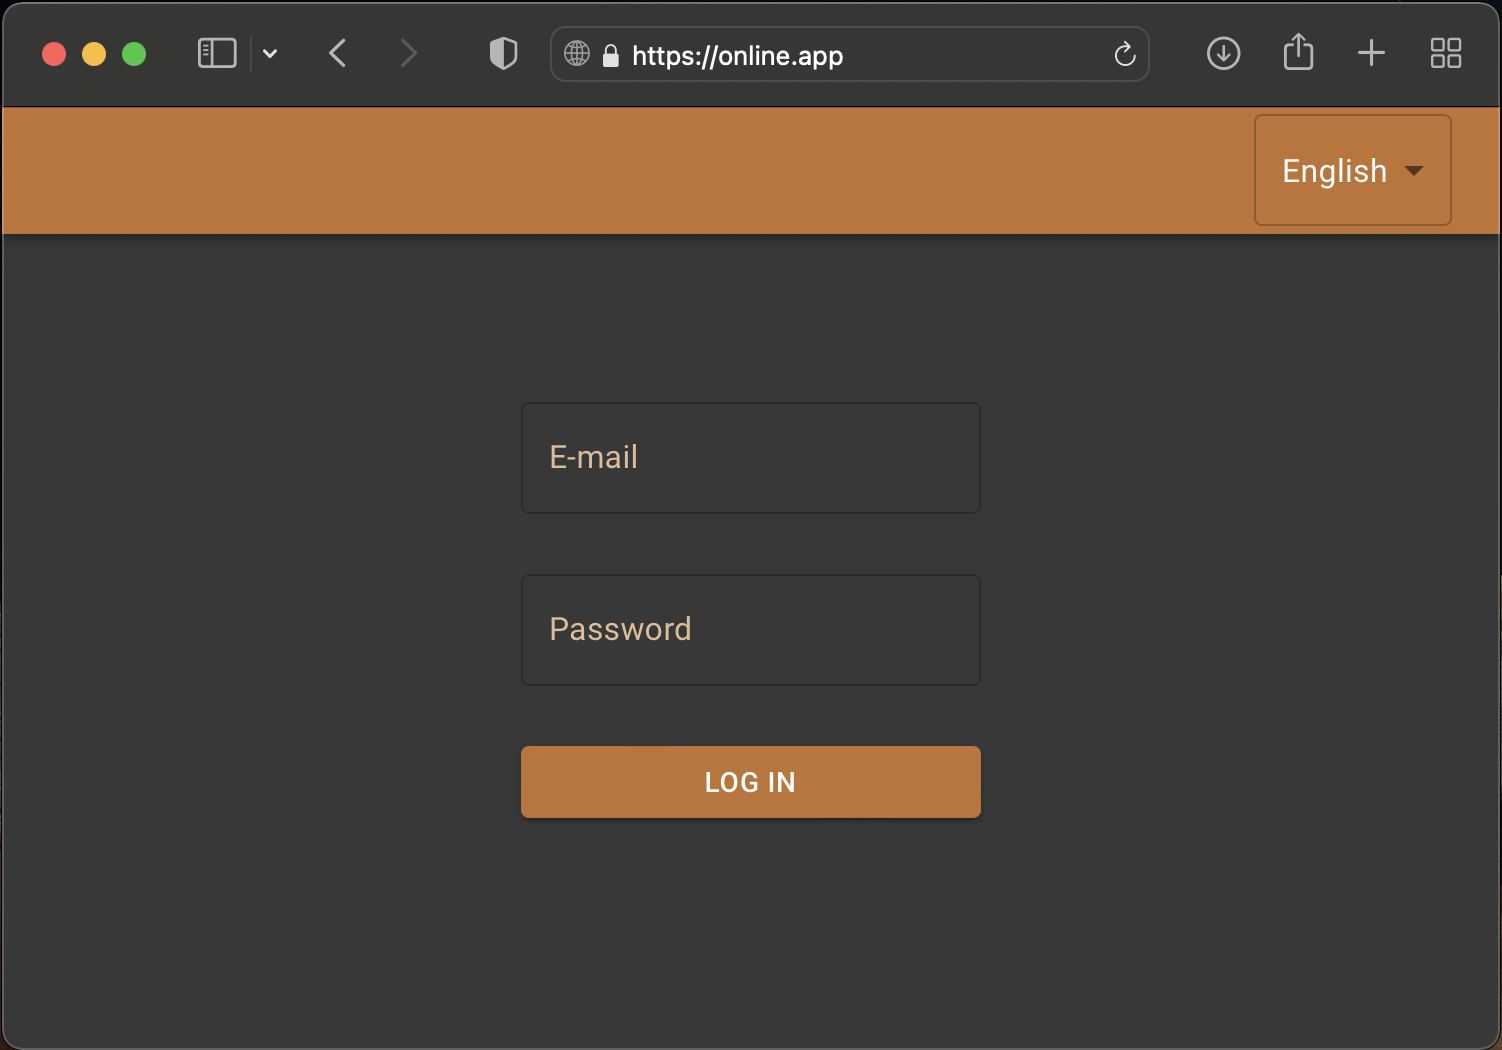
\includegraphics[scale=0.4]{src/figures/app-screen}
    \caption{Скриншот открытия страницы веб-сервиса}
    \label{fig:app-screen}
\end{figure}

%%% Local Variables:
%%% mode: latex
%%% TeX-master: "rpz"
%%% End:

    \chapter{Экспериментальный раздел}
\label{cha:research}

В данном разделе проводятся вычислительные эксперименты.
А на рис.~\ref{fig:spire01} показана схема мыслительного процесса автора...

\begin{figure}
    \centering
    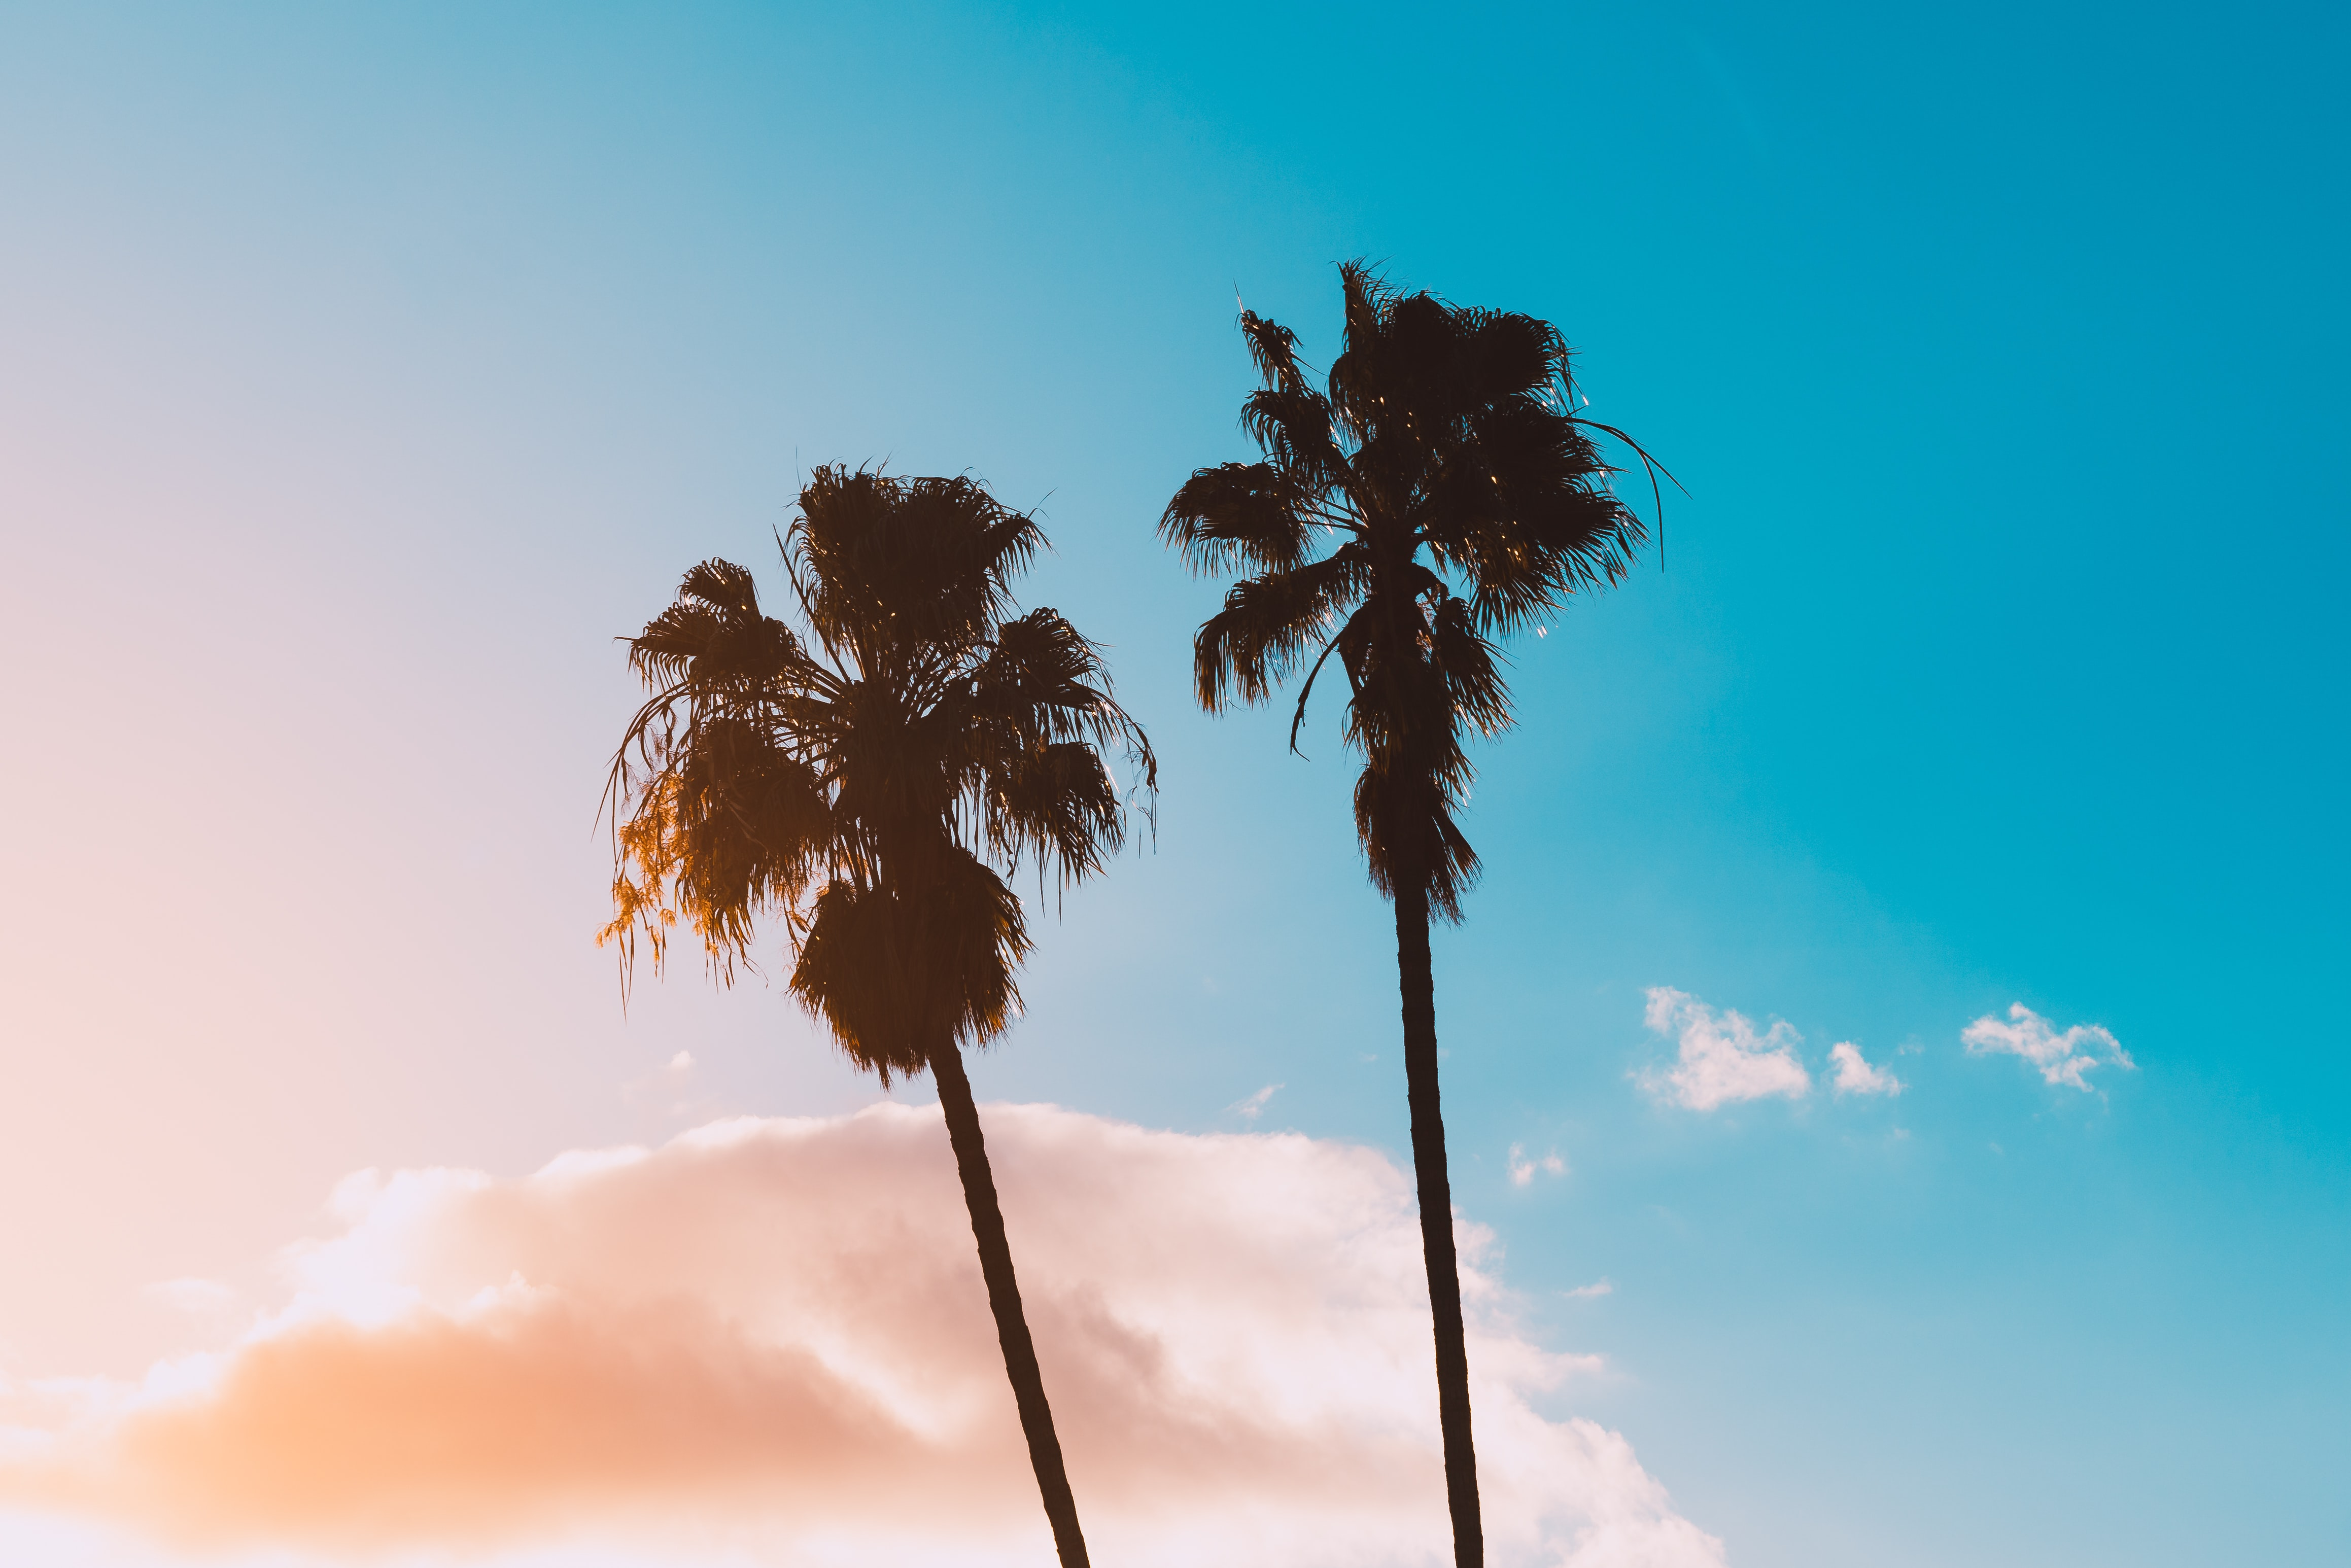
\includegraphics[scale=0.1]{figures/pic01}
    \caption{Как страшно жить}
    \label{fig:spire01}
\end{figure}


%%% Local Variables:
%%% mode: latex
%%% TeX-master: "rpz"
%%% End:


    \backmatter %% Здесь заканчивается нумерованная часть документа и начинаются ссылки и
    %% заключение

    \Conclusion % заключение к отчёту

Результаты выполнения задания на выпускную квалификационную работу, - позволяют сделать следующие выводы:
\begin{itemize}
    \item
    Цель исследования: развернуть и автоматизировать управление жизненным циклом веб-сервиса на базе Node.js, - полностью реализована;
    вариант предложенного решения развёртывания позволяет быстро ввести веб-сервис на базе Node.js в рабочее состояние и автоматизировать управление его жизненным циклом по современным методологиям DevOps.

    \item
    В рамках решения задачи: Провести обзор необходимых средств для автоматизации управления жизненным циклом веб-сервиса,
    - были рассмотрены преимущества системы контроля версий Git, проанализированы основные технические параметры и отличия между различными Git хостингами, а так же инструментами оркестрации контейнеров Docker Swarm и Kubernetes .

    \item
    В рамках решения задачи: Рассмотреть полученный для развёртывания веб-сервис и проанализировать требования,
    - была составлена и описана диаграмма развёртывания веб-сервиса, была установлена необходимость хранилища пакетов и образов, были описаны актёры и случаи использования системы в виде соответствующей диаграммы.

    Отдельно были описаны рабочие окружения веб-сервиса и на основании необходимых для развёртывания компонентах были составлены виды репозиториев в системе.

    \item
    В рамках решения задачи: Провести проектирование механизмов автоматизации управления жизненного цикла веб-сервиса,
    - были выбраны и автоматизированы два основных вида тестирования веб-сервиса с предоставлением аналитических данных сотрудникам отдела качества,
    была составлена и задокументирована диаграмма компонентов конфигураций внутри репозиториев системы.

    Отдельное внимание было уделено применению модели ветвления Git Flow вместе с инструментами автоматизации CI/CD в целях автоматизированного создания релизов сервисов и библиотек,
    а так же нахождению компонентов для обновления при помощи обхода графа зависимостей.

    Так же была спроектирована диаграмма компонентов репозиториев для организации хранения исходного кода отдельно от конфигурационных файлов развёртки веб-сервиса.

    \item
    В рамках решения задачи: Составить план тестирования механизмов развёртывания веб-сервиса,
    - были сформулированы цели и задачи тестирования, была выбрана методология тестирования, а так же были описаны тестовые сценарии.

    \item
    В рамках решения задачи: Провести практические работы по развёртке и автоматизации управления жизненного цикла веб-сервиса,
    - в GitLab была создана группа проекта, были созданы необходимые репозитории согласно диаграммам и загружен исходный код веб-сервиса.

    На рабочем сервере были открыты TCP и UDP порты, а так же были введены требуемые команды для инициализации кластера Docker Swarm.
    Отдельно был зарегистрирован GitLab Runner и сконфигурирован под оптимальную работу с кешированием в системе.

    \item
    В рамках решения задачи: Провести тестирование механизмов развёртывания и обосновать полученные результаты,
    - было произведено ручное тестирование по методологии <<Белого ящика>> функций полученной системы.
\end{itemize}


%%% Local Variables:
%%% mode: latex
%%% TeX-master: "rpz"
%%% End:

    % % Список литературы при помощи BibTeX
% Юзать так:
%
% pdflatex rpz
% bibtex rpz
% pdflatex rpz

\bibliographystyle{src/styles/gost780u}
\bibliography{src/rpz}

%%% Local Variables:
%%% mode: latex
%%% TeX-master: "rpz"
%%% End:


    \appendix   % Тут идут приложения
%
%    \chapter{Картинки}
\label{cha:appendix1}

\begin{figure}
    \centering
    \caption{Картинка в приложении. Страшная и ужасная.}
\end{figure}

%%% Local Variables: 
%%% mode: latex
%%% TeX-master: "rpz"
%%% End: 

%    \chapter{Еще картинки}
\label{cha:appendix2}

\begin{figure}
    \centering
    \caption{Еще одна картинка, ничем не лучше предыдущей. Но надо же как-то заполнить место.}
\end{figure}

%%% Local Variables: 
%%% mode: latex
%%% TeX-master: "rpz"
%%% End: 


\end{document}

%%% Local Variables:
%%% mode: latex
%%% TeX-master: t
%%% End:
